\documentclass[12pt,a4paper]{article}
\usepackage[utf8]{inputenc}
\usepackage[german]{babel}
\usepackage[T1]{fontenc}
\usepackage{times}
\usepackage{graphicx}
\usepackage{url}
\usepackage{color}
\usepackage{setspace}
\usepackage{enumerate}
\usepackage{amsmath}
\usepackage{amsfonts}
\usepackage{amssymb}
\usepackage{float}
\usepackage{stix}
\usepackage{xcolor}
\newcommand{\red}[1]{\textcolor{red} {#1}}
\newcommand{\blue}[1]{\textcolor{blue} {#1}}
\newcommand{\green}[1]{\textcolor{green} {#1}}
\newcommand{\yellow}[1]{\textcolor{yellow} {#1}}
\newcommand{\nl}{\\[0.1cm]}
\title{Zusammenfassung Software-orientierte Informatik}
\author{Henrik Tscherny}
\begin{document}
\maketitle
\tableofcontents

\section{Systeme}
Ein System ist ein natürliches oder künstliches Gebilde, welches aus Eingangssignalen ($E$) ein Ausgangssignal ($A$) macht. Das System besitzt zudem einen inneren Zustand, der durch Zustandsgrößen ($\vec{Z}$) beschrieben wird. Eine Systemfunktion ($F$) legt fest wie das Eingangssignal in das Ausgangssignal umgewandelt wird ($\vec{A} = F(\vec{E}, \vec{Z},...)$)

\paragraph{Statische Systeme}
Der Output zum Zeitpunkt t ($y(t)$) ist nur von dem zu gleichen Zeitpunkt am Input anliegenden Wert ($x(t)$) abhängig. Innere Zustände ($\vec{Z}$) sind egal. die dazugehörige Funktion $y=f(x)$ nennt man statische Kennlinie.

\paragraph{Dynamische Systeme}
Der Output ($y(t)$) ist von dem am Input anliegenden Signal ($x(t)$) und dem inneren Zustand des Systems ($\vec{Z}$) abhängig. Dabei kann man sich den inneren Zustand als eine Art Gedächtnis vorstellen

\paragraph{Lineare Systeme}
Ein System ist linear, wenn der Überlagerungssatz/Superpositionsprinzip gilt, bzw nicht-linear falls dieser nicht gilt.\\
$f(x_1 + x_2) = f(x_1) + f(x_2) \Rightarrow y(t) = f(x_1(t) + x_2(t)) = f(x_1(t)) + f(x_2(t))$\\
lineare Systeme werden durch lineare Differenzialgleichungen mit konstanten Koeffizienten beschrieben

\paragraph{Zeit(in)variante Systeme}
Ändern sich die Systemeigenschaften sich nicht mit der Zeit, d.h. es gilt das Verschiebungsprinzip ($y(t-t_0) = f(x(t-t_0))$), ist das System zeitinvariant, andernfalls ist es zeitvariant

\paragraph{Kausales System}
Der Output ist nur von den aktuellen und vergangenen Inputs abhängig, Sprung- und Impulsantwort sind gleich 0 für $t < 0$, gilt dies nicht ist das System akausal.
\begin{itemize}
\item schwach kausal
\begin{itemize}
\item reagiert auf Input x immer mit gleichem Output y
\end{itemize}
\item stark kausal
\begin{itemize}
\item reagiert auf ähnlichen Input x mit ähnlichem Output y
\end{itemize}
\end{itemize}

\subsection{Verknüpfung von Systemen}

\paragraph{Reihenschaltung}
\hspace{1pt}
\begin{figure}[H]
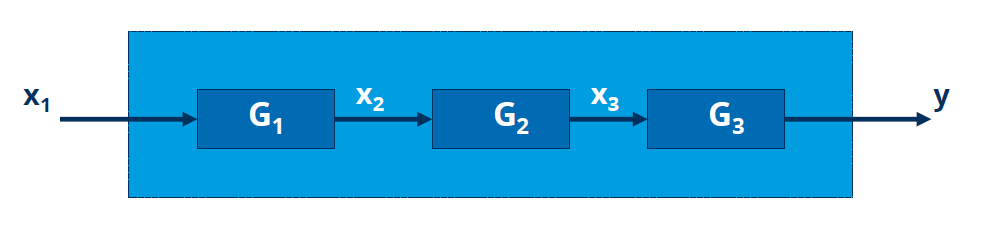
\includegraphics[scale=0.5]{./resources/reihenschaltung.png}
\end{figure}
\begin{tabular}{|c|c|}
\hline
\textbf{statisches System} & \textbf{dynamisches System} \\
$\displaystyle k_{ges} = \prod_{i=1}^n k_i = \frac{\text{output}}{\text{input}}$ & $\displaystyle G_{ges}(f) = \prod_{i=1}^n G_i(f) = \frac{\text{input}(f)}{\text{output}(f)}$ \\
\hline
$G_i = k_i$: statische Übertragungsfaktor & $G_i(f)$: Übertragungsfunktion des Teilsystems i \\
\hline
\end{tabular}
\newpage
\paragraph{Parallelschaltung}
\hspace{1pt}
\begin{figure}[H]
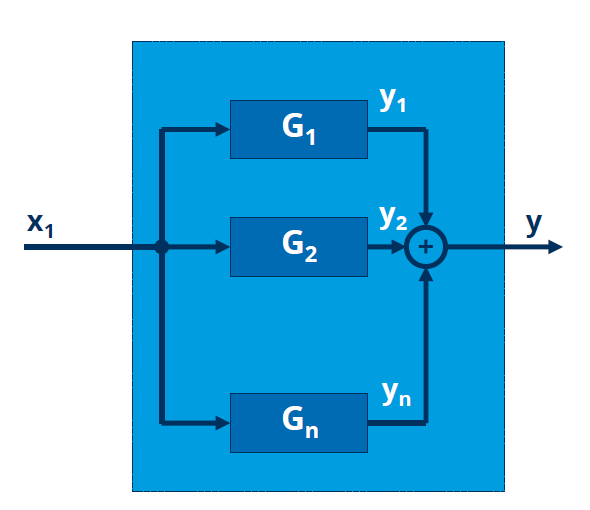
\includegraphics[scale=0.5]{./resources/parallelschaltung.png}
\end{figure}
\begin{tabular}{|c|c|}
\hline
\textbf{statisches System} & \textbf{dynamisches System} \\
$\displaystyle k_{ges} = \sum_{i=1}^n k_i$ & $\displaystyle G_{ges}(f) = \sum_{i=1}^n G_i(f)$\\
\hline
$G_i = k_i$: statische Übertragungsfaktor & $G_i(f)$: Übertragungsfunktion des Teilsystems i \\
\hline
\end{tabular}

\paragraph{Rückkopplungsschaltung}
\hspace{1pt}
\begin{figure}[H]
\includegraphics[scale=0.5]{./resources/rückkopplungsschaltung.png}
\end{figure}
\begin{tabular}{|c|c|}
\hline
\textbf{statisches System} & \textbf{dynamisches System} \\
$\displaystyle k_{ges} = \frac{y}{x} = \frac{k_1}{1 \pm k_1 k_2}$ & $\displaystyle G_{ges}(f) = \frac{G_1(f)}{1 \pm G_1(f)G_2(f)}$\\
\hline
\end{tabular}

\end{document}